\documentclass{article}
\title{Computer simulations of Stochastic Processes}
\author{Adam Janik}

\usepackage{amsmath}

\usepackage{ifthen,xcolor}
\newlength{\tabcont}

\newcommand{\tab}[1]{%
\settowidth{\tabcont}{#1}%
\ifthenelse{\lengthtest{\tabcont < .25\linewidth}}%
{\makebox[.25\linewidth][l]{#1}\ignorespaces}%
{\makebox[.5\linewidth][l]{\color{red} #1}\ignorespaces}%
}%

\usepackage{listings}
\usepackage{color}
\usepackage{graphicx}
\usepackage{amssymb}

\definecolor{dkgreen}{rgb}{0,0.6,0}
\definecolor{gray}{rgb}{0.5,0.5,0.5}
\definecolor{mauve}{rgb}{0.58,0,0.82}

\lstset{frame=tb,
  language=Matlab,
  aboveskip=3mm,
  belowskip=3mm,
  showstringspaces=false,
  columns=flexible,
  basicstyle={\small\ttfamily},
  numbers=none,
  numberstyle=\tiny\color{gray},
  keywordstyle=\color{blue},
  commentstyle=\color{dkgreen},
  stringstyle=\color{mauve},
  breaklines=true,
  breakatwhitespace=true,
  tabsize=4
}

\newcommand\xput[2][0.5]{%
    \rule{#1\linewidth}{0pt}\makebox[0pt][c]{#2}\hfill}


\begin{document}
	\pagenumbering{gobble}
	\maketitle
	\newpage
	\pagenumbering{arabic}
	
	\section{Introduction}
	In this report we are going to discuss and present some aspects regarding simulating stochastic processes. A couple of scripts has been attached to this document - they were used to produce plots and results in this report.
	\section{Stable distribution}
	In particular, we will discuss here stable distributions - a class of probability distributions, that allow skewness and heavy tails, and so have a lot of interesting mathematical properties, as well as many applications in finance, insurance mathematics, biology and many more.
	In general, an univariate stable random variables are characterized by four parameters:
	\begin{itemize}
	\item $\alpha$ - the most important one, called index of stability
	\item $\sigma$ - scale parameter
	\item $\beta$ - skewness parameter
	\item $\mu$ - shift parameter
	\end{itemize}
	Those parameters will be discussed later, here we can mention that if we want to receive Gaussian distribution, we put $\alpha = 2$, $\beta = 0$, and so $\mu$ will be mean and $\sigma$ - standard deviation.
	\subsection{Definition}
	We define $X$ as stable distribution if it holds the following property\footnote{Nolan J. P., "Stable Distributions. Models for Heavy Tailed Data", http://academic2.american.edu/~jpnolan/stable/stable.html}
	\begin{equation}
	aX_1+bX_2 \stackrel{d}{=} cX + d
	\end{equation}
	where $a, b$ and $c$ are positive, $d\in R$ and $X_1, X_2$ are independent copies of $X$.
	However, there is also another representation of stable random variable; we can say, that random variable $X$ is stable if and only if $X \stackrel{d}{=} aZ + b$ witch $Z$ being random variable with characteristic function:
	\begin{equation}
		\mathbf{E} \exp(i\mu Z) = \begin{cases}
		\exp(|\mu|^\alpha[1-i\beta \tan\frac{\pi \alpha}{2}(\mbox{sign}\mu)]) & \alpha \neq 1 \\
		\exp(|\mu|[1+i\beta \frac{2}{\pi} (\mbox{sign}\mu) \log |\mu|]) & \alpha = 1
		\end{cases}
	\end{equation}
In this equation we have $0<\alpha \leq 2$ and $-1 \leq \beta \leq 1$, $a$ must be different than $0$ and $b$ is a real number.\\
A more precise description and derivation of stable distribution can be found in dedicated literature\footnote{Samorodnitsky G, Taqqu M.S, "Stable Non-Gaussian Random Processes"}. Here we are going to discuss some aspect of simulations and properties.

	\subsection{Simulation and properties}
	A simple function (for Matlab language) to simulate stable random variables\footnote{Borak, Hardle, Weron, 2005} has been attached to this report. Crucial for us is to check if it works correctly and investigate properties of the simulated distribution. Fortunately, a there is a very well-known program\footnote{http://academic2.american.edu/~jpnolan/stable/stablec.exe}, written by John P. Nolan, available on his website. With it's help, we will be able to test our function.
	\subsubsection{Testing for correctness of the function}
	Let's make four calls of the function to generate data, and then check if with Nolan's program:
	\begin{lstlisting}
	gaussian = stable(2, 0, 1, 0, 100000);$
	cauchy = stable(1, 0, 1, 0, 100000);$
	levy = stable(0.5, 1.0, 1, 0, 100000);$
	distr = stable(1.3, 0.3, 2, -5, 100000);$
	\end{lstlisting}
	As a result, we obtained four samples of stable distribution; now we can check them with Nolan's program. We choose each time maximum likelihood estimators of parameters method to get parameters based on sample. \\
	
	For a variable \textit{gaussian} the output is:
	\begin{lstlisting}
	 Stable model with maximum likelihood estimator
	 
  Initial quantile estimate of S0 parameters
         alpha     beta      gamma         delta
      2.000000}  0.000000    1.00421       0.911811E-03   
\end{lstlisting}       
   
For a variable \textit{cauchy} the output is:
\begin{lstlisting}
	 Stable model with maximum likelihood estimator
	 
  Initial quantile estimate of S0 parameters
         alpha      beta      gamma         delta
      0.995880  -0.017271    1.00109       0.190453E-02
\end{lstlisting} 

For a variable \textit{levy} the output is:\\
\begin{lstlisting}
	 Stable model with maximum likelihood estimator
	 
  Initial quantile estimate of S0 parameters
         alpha      beta      gamma         delta
      0.506668  0.815349    1.31190       1.17643   
\end{lstlisting} 

For a variable \textit{distr} the output is:
\begin{lstlisting}
	 Stable model with maximum likelihood estimator
	 
  Initial quantile estimate of S0 parameters
         alpha      beta      gamma         delta
      1.306687  0.311575    1.99745       -6.18514   
\end{lstlisting}  
We can say here now, that estimation goes worse as $\alpha$ is going lower - especially for $\mu$ (or - in other sources $\sigma$) parameter; we should be careful when we are saying something about shift parameter, when we operating on the low-$\alpha$ samples.

	\begin{figure}[h]
		\xput[0.5]{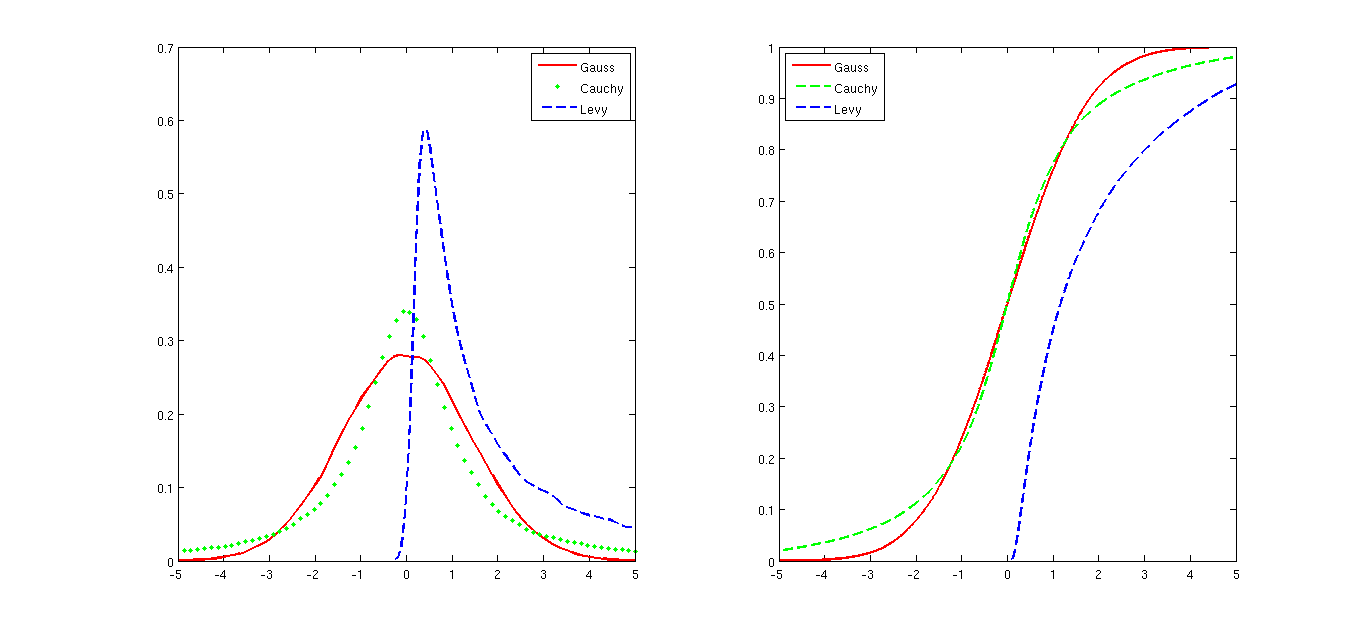
\includegraphics[width=1.7\linewidth]{gauss_cauchy_levy}}
		
		\caption{Simulated three important distributions with $\alpha = 2, 1, 0.5$}
	\end{figure}

\subsection{Description of the parameters}
In this subsection we will discuss each of the parameters and how changing them, impacts obtained sample.
\subsubsection{$\alpha$ parameter}
Mentioned before, index of stability is often referred as the most important one. On the Figure 2 three samples have been presented, to illustrate how stable distribution behave with decreasing $\alpha$. We can see that three things occur to the density: peak gets higher, the region flanking peak get lower, and - what makes stable distribution such important and interesting - the tails gets heavier.\\
As shown in the next section, $\alpha$ affects heavily other parameters.

	\begin{figure}[h]
		\xput[0.5]{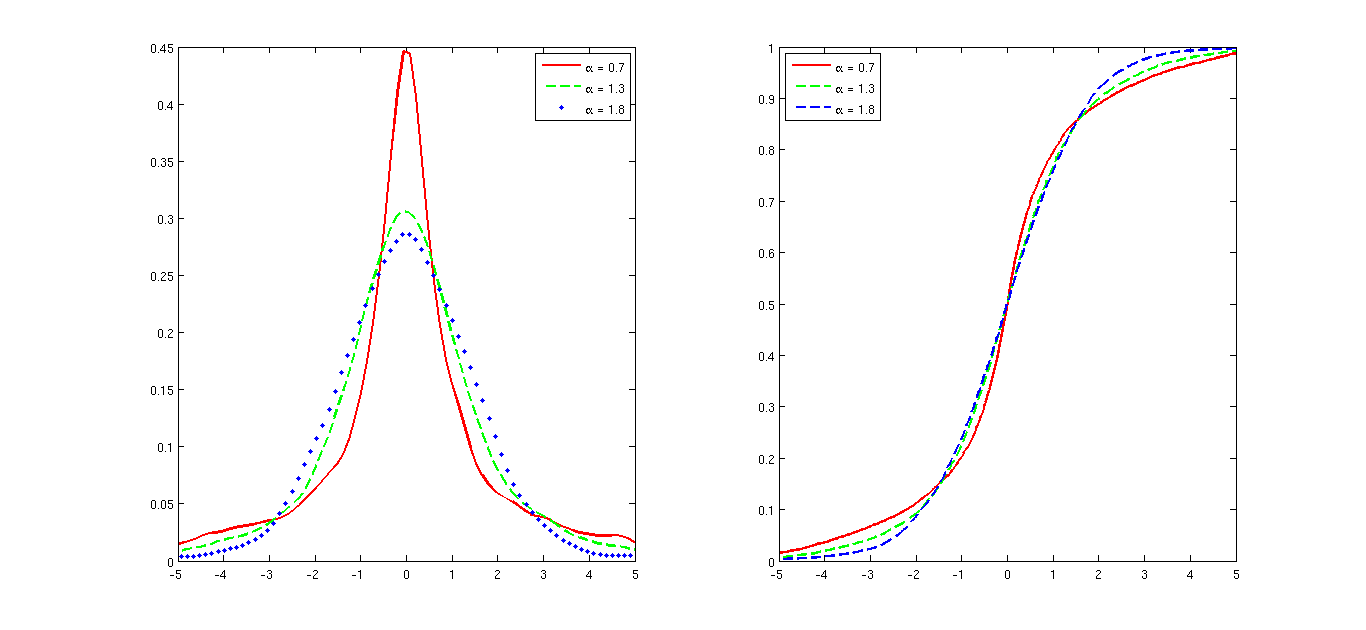
\includegraphics[width=1.5\linewidth]{stable_param_alpha}}
		
		\caption{Stable distribution pdf and empirical cdf for $\alpha = 0.7, 1.3, 1.8$}
	\end{figure}

\subsubsection{$\beta$ parameter}
Three different plots for different simulated samples will be needed, to show how $\beta$ influence our distribution.

Figure 3 allows us to see, that with increasing $\beta$, the distribution becomes more and more skewed to the right (in case of $\beta$ negative, we would see similar behavior, but to the left side)
	\begin{figure}[h]
		\xput[0.5]{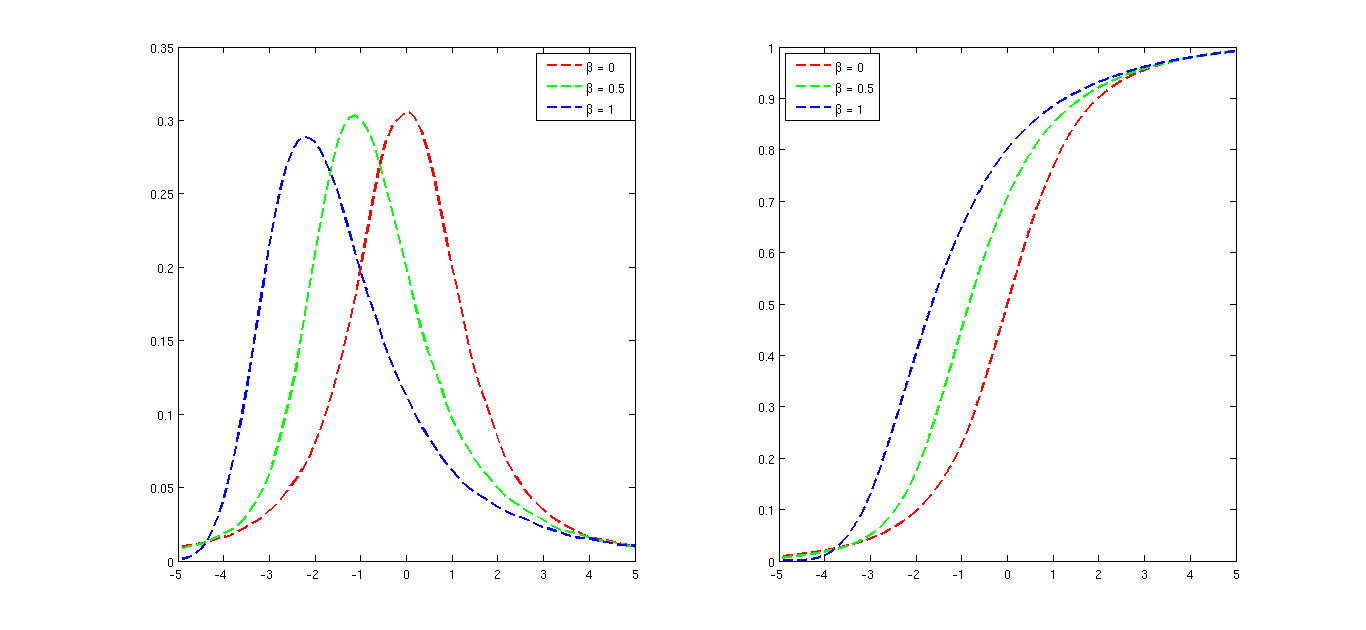
\includegraphics[width=1.5\linewidth]{stable_param_beta13}}
		
		\caption{Stable distribution pdf and empirical cdf for $\alpha = 1.3$ and $ beta = 0, 0.5, 1$}
	\end{figure}
\newpage
In Figures 4 and 5 $\beta$ varying in the same way, but samples has been simulated for $\alpha = 1$ and $\alpha = 0.7$ respectively.
	\begin{figure}[h]
		\xput[0.5]{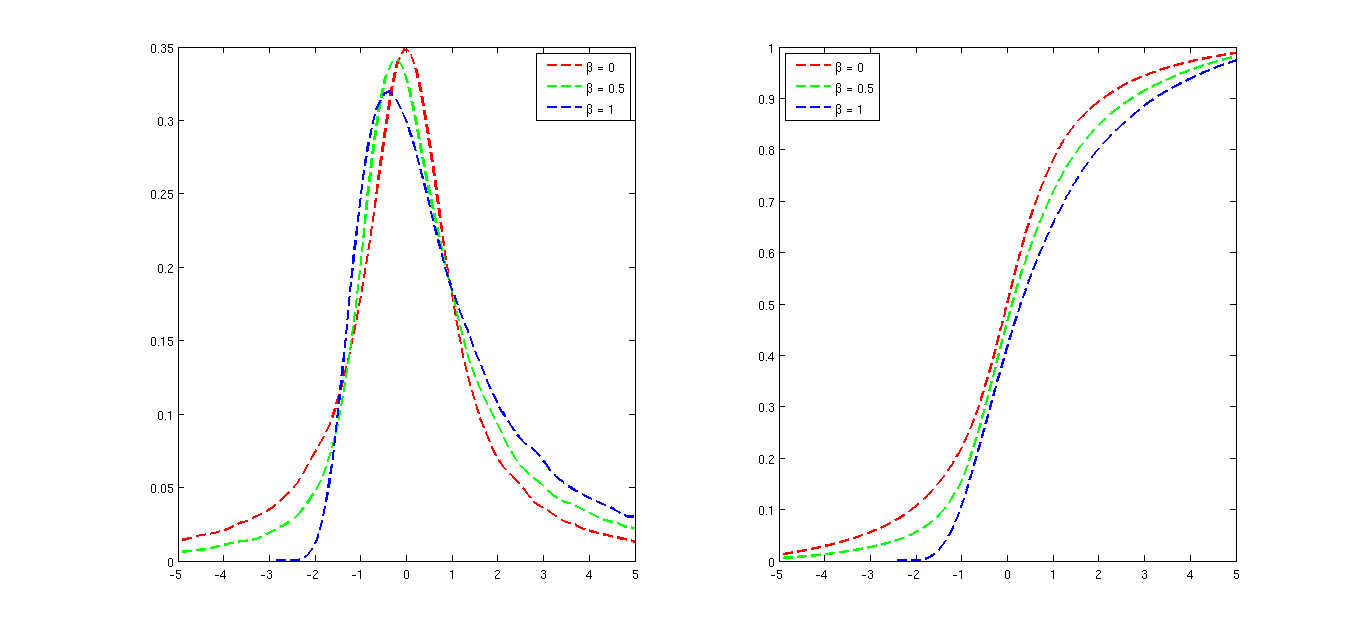
\includegraphics[width=1.5\linewidth]{stable_param_beta10}}
		
		\caption{Stable distribution pdf and empirical cdf for $\alpha = 1$ and $ beta = 0, 0.5, 1$}
	\end{figure}
	
	\begin{figure}[h]
		\xput[0.5]{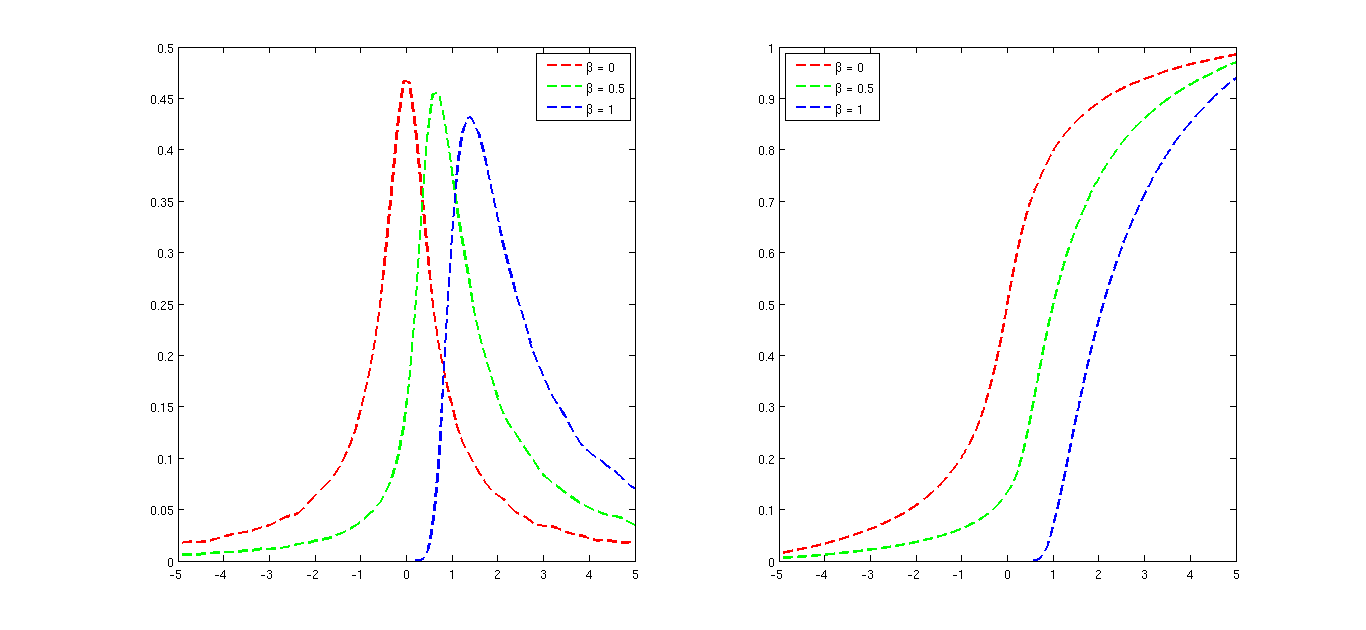
\includegraphics[width=1.5\linewidth]{stable_param_beta07}}
		
		\caption{Stable distribution pdf and empirical cdf for $\alpha = 0.7$ and $ beta = 0, 0.5, 1$}
	\end{figure}
We see that with decreasing $\alpha$, $\beta$ becomes more and more significant, making distribution more and more skewed, until it reach 1 (-1) - then we say that distribution is \textit{totally skewed to the right (left)}. It can also be shown, that for $\alpha < 1$ and $|\beta| = 1$ the whole weight is in one of the tails (depending if $\beta$ is negative or positive).

\clearpage

\subsubsection{$\sigma$ and $\mu$ parameters}
Here we briefly take a look for remaining two parameters. $\sigma$ tells us about how spread distribution is, while $\mu$ - where the "center" of the parameter is. For a Gaussian distribution we call them \textit{variance} and \textit{mean} respectively, however, we should generally avoid those terms, as they may not exist according to mathematical definitions.
	\begin{figure}[h]
		\xput[0.5]{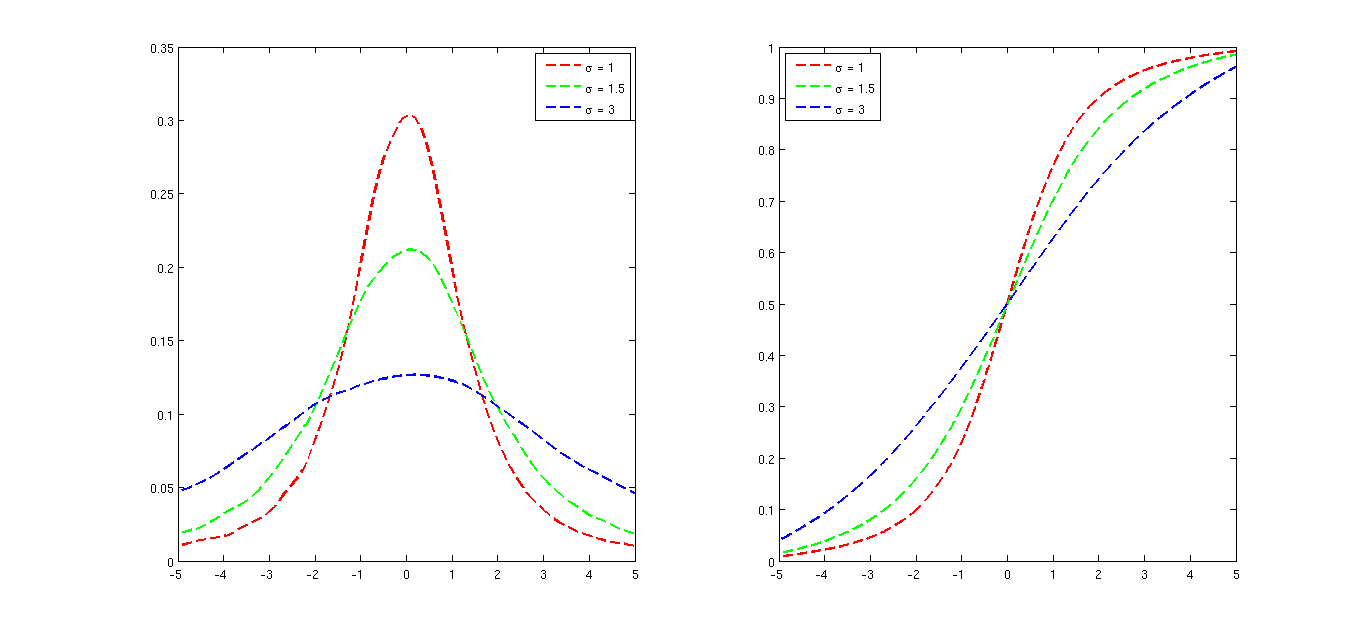
\includegraphics[width=1.2\linewidth]{stable_param_sigma}}
		
		\caption{Stable distribution pdf and empirical cdf for $\alpha = 1.3$ and $ sigma = 1, 1.5, 3$}
	\end{figure}
\newpage
	\begin{figure}[h]
		\xput[0.5]{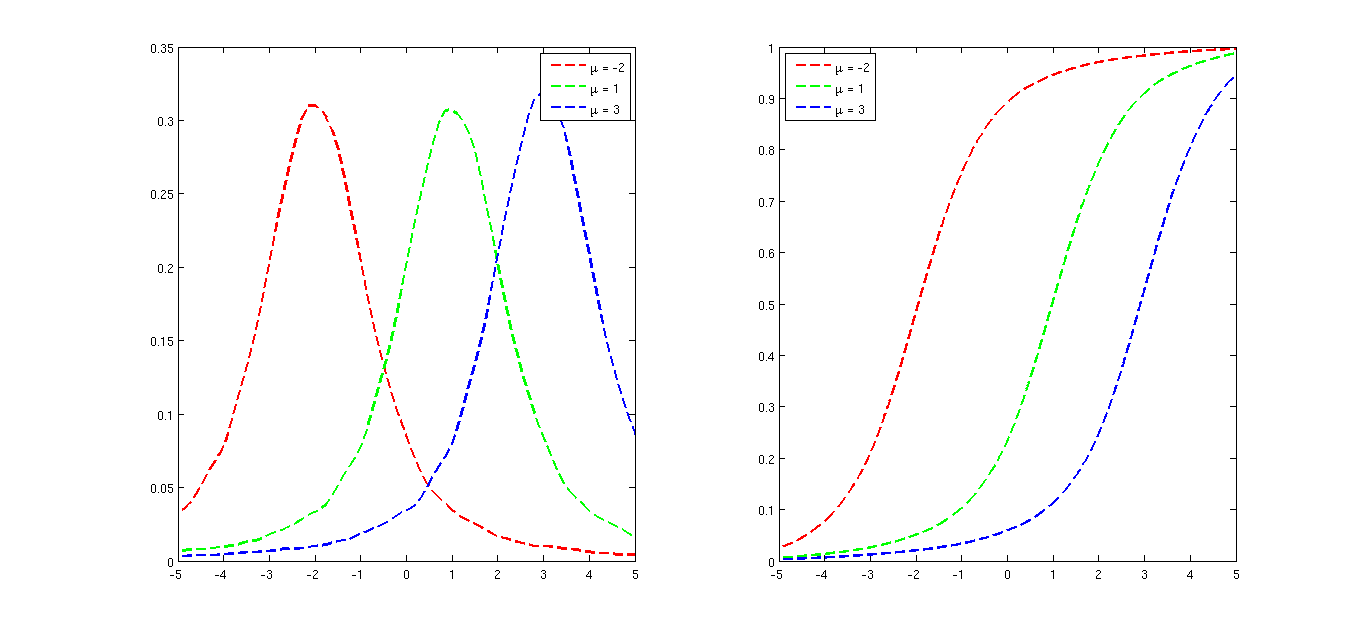
\includegraphics[width=1.2\linewidth]{stable_param_mu}}
		
		\caption{Stable distribution pdf and empirical cdf for $\alpha = 1.3$ and $ mu = -2, 1, 3$}
	\end{figure}

\subsection{Properties}
Here we discuss some of the commonly known properties\footnote{Samorodnitsky G, Taqqu M.S, "Stable Non-Gaussian Random Processes"} of the stable distributions.
\subsubsection{Property 1 - sum of stable random variables}
First, we are going to study the following property\footnote{Samorodnitsky G, Taqqu M.S, "Stable Non-Gaussian Random Processes"}:
\subparagraph{Property 1}
\textit{Let $X_1$ and $X_2$ be independent stable random variables, $X_i \sim S_\alpha(\beta_i, \sigma_i, \mu_i)$, $i = 1,2$. Then $X_1 + X_2 \sim S_\alpha(\beta, \sigma, \mu)$, with: }
\begin{equation}
\sigma = (\sigma_1^\alpha + \sigma_2^\alpha)^{1/\alpha}, \qquad \mu = \mu_1 + \mu_2, \qquad \beta = \frac{\beta_1\sigma_1^\alpha + \beta_2\sigma_2^\alpha}{\sigma_1^\alpha + \sigma_2^\alpha}
\end{equation}
Following code has been ran to simulate two samples:

\begin{lstlisting}
alpha = 1.8;
mu1 = 1; mu2 = 0.5;
sigma1 = 0.5; sigma2 = 0.3;
beta1 = 0.3; beta2 = 0.8;
sigma = ( sigma1^alpha + sigma2^alpha )^(1/alpha);
beta = ( beta1*(sigma1^alpha) + beta2*(sigma2^alpha) ) / ( sigma1^alpha + sigma2^alpha );
mu = mu1 + mu2;

X1 = stable(alpha, beta1, sigma1, mu1, 10000000);
X2 = stable(alpha, beta2, sigma2, mu2, 10000000);
X = X1 + X2;
save X.txt X -ascii;
\end{lstlisting}
Values computed according to formula above are as follows: $sigma = 0.6025, \beta = 0.4425, \mu = 1.5000$; output from Nolan's program, checking parameters:
\begin{lstlisting}
  Initial quantile estimate of S0 parameters
         alpha      beta      gamma         delta
      1.800206  0.452978   0.602503        1.41195 
\end{lstlisting}   
The largest difference between theoretical and simulated value is at $\delta$ (or $\mu$) parameter; however, taking consideration, that in the previous examples it was most variable parameter, we can say that property holds.

\subsubsection{Property 2}
Another property, that we can easily check is the following one
\subparagraph{Property 2}
For any $0 < \alpha < 2$,
\begin{equation}
X \sim S_\alpha(\beta, \sigma, \mu) \iff -X \sim S_\alpha(-\beta, \sigma, \mu)
\end{equation}

\begin{lstlisting}
alpha = 1.8; mu = 0; sigma = 1; beta = 0.7;
X = stable(alpha, beta, sigma, mu, 1000000);
X = -X; save X.txt X -ascii;
\end{lstlisting} 
And again we check with the Nolan's program:
\begin{lstlisting}
  Initial quantile estimate of S0 parameters
         alpha      beta      gamma         delta
      1.802983 -0.716207    1.00018       0.230816 
\end{lstlisting}
We can say that property holds.

\subsubsection{Property 3 - series representation}
We are going to show now, that $\alpha$-stable random variable can be represented as a convergent sum of random variables involving arrival times of a Poisson process.\\
We consider stable process for $0 < \alpha < 0$. Let's denote $N_\delta$ - Poisson r.v. with parameter $\delta$. We need to introduce a new r.v. with distribution function:
	\begin{equation*}
		P(Y_{\delta, k}) = \begin{cases}
		\delta^\alpha X^{-\alpha} & X > \delta \\
		1 & X < \delta
		\end{cases}
	\end{equation*}
Now, if we look at the following variable:
\begin{equation*}
X_\delta = \sum_{k>1}^{N_j} Y_{j,k}
\end{equation*}
We can say, that $X_\delta$ for $\delta$ going to 0 becomes $\alpha$ subordinator - stable r.v. with parameters $S(\alpha, \sigma, 1, 0)$ with:
\begin{equation*}
\sigma^\alpha = \Gamma(1 - \alpha)cos(\pi \frac{\alpha}{2})
\end{equation*}
Figure 8 shows how tails of the distribution converges to stable distribution (blue line is $S(\alpha, \sigma, 1, 0)$).
	\begin{figure}[h]
		\xput[0.5]{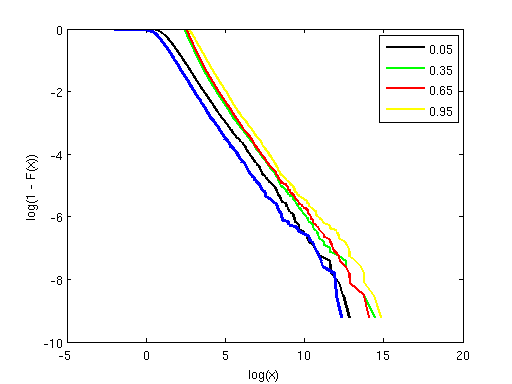
\includegraphics[width=1.2\linewidth]{stablesubordin}}
		
		\caption{Tails of stable subordinators for different $\delta$ on double log scale; $\alpha = 0.7$ here.}
	\end{figure}

\section{Multivariate stable distributions}
An logic step forward is to simulate and investigate multivariate stable distributions. We will briefly note important facts about them, and then present method of simulation and results.
\subsection{Characterization}
We use $\mathbf{X}$ to denote $d$-dimensional $\alpha$-stable random vector determined by the spectral measure $\Gamma$ (a finite Borel measure on $S_d$ = unit sphere in $\mathbb{R}$) and a shift vector $\mu^0 \in \mathbb{R}^d$. The characteristic function of $\mathbf{X}$ is:
\begin{equation}
\psi_{\mathbf{X}}(\mathbf{t}) = \mathbf{E}\exp\{i< \mathbf{X}, \mathbf{t} >\} = \exp(-I_\mathbf{X}(\mathbf{t}) + i < \mu^0, t>)
\end{equation}
Where $I_\mathbf{X}$ is:
\begin{equation}
I_\mathbf{X}(\mathbf{t}) = \int_{S_d}\psi_\alpha(<\mathbf{t}, \mathbf{s}>)\Gamma(ds)
\end{equation}
and $\psi_\alpha$:

	\begin{equation}
		\psi_\alpha(u) = \begin{cases}
		|u|^{\alpha}(1 - i \mbox{sign}(u) \tan(\frac{\pi \alpha}{2}) & \alpha \neq 1 \\
		|u|(1 - i \frac{2}{\pi}\mbox{sign}(u) \log(|u|) & \alpha = 1
		\end{cases}
	\end{equation}

\subsection{Simulation}
For simulation, we consider $\Gamma$ as a discrete spectral measure with finite number of point masses:
\begin{equation}
\Gamma( \cdot ) = \sum_{j=1}^n \gamma_j \delta_{\mathbf{s}_{j}}( \cdot )
\end{equation}
Where $\gamma_j$'s are weights and $\delta_\mathbf{s_{j}}$'s are point masses at the point $\mathbf{s_j} \in S_d$. With that knowledge, we can define method for simulating random vectors\footnote{[3]}:
	\begin{equation}
		\mathbf{X} \stackrel{D}{=} \begin{cases}
		\sum_{j=1}^{n} \gamma_{j}^{1/\alpha} Z_j \mathbf{s}_j & \alpha \neq 1 \\
		\sum_{j=1}^{n} \gamma_{j} (Z_j + \frac{2}{\pi}\log \gamma_j) \mathbf{s}_j & \alpha = 1
		\end{cases}
	\end{equation}
To test algorithm, we will try to retrieve contour plots from J. Nolan's paper; after setting the variables (whole procedure in \textit{multi.m} file):
\begin{lstlisting}
gam1 = 0.25; s1 = [1, 0]; 
gam2 = 0.125; s2 = [0.5, sqrt(3)/2];
gam3 = 0.25; s3 = [-0.5, sqrt(3)/2];
gam4 = 0.25; s4 = [-1, 0];
gam5 = 0.125; s5 = [-0.5, -sqrt(3)/2];
gam6 = 0.25; s6 = [0.5, -sqrt(3)/2];
\end{lstlisting} 
And similar for second case, we obtain plots as in Figure 9 and 10.
	\begin{figure}[h]
		\xput[0.5]{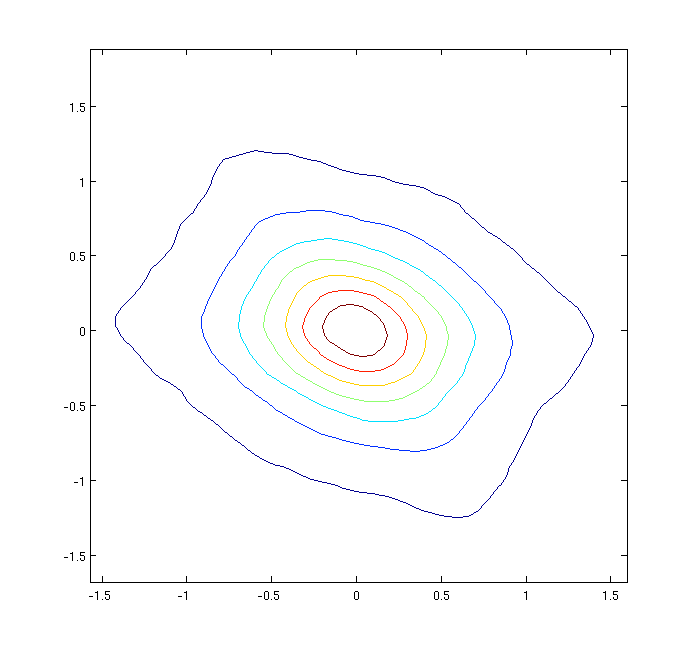
\includegraphics[width=0.75\linewidth]{multi_contour1}}
		
		\caption{Two dimensional symmetric stable curves with $\alpha = 0.9$}
	\end{figure}
	\begin{figure}[h]
		\xput[0.5]{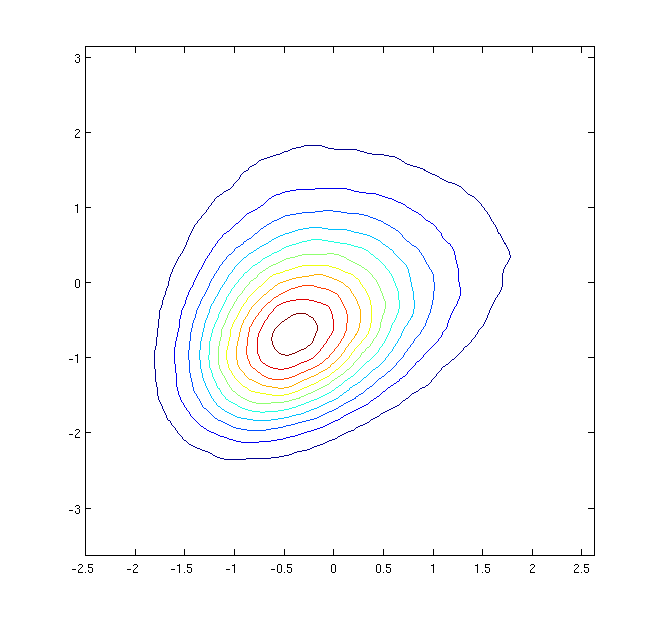
\includegraphics[width=0.75\linewidth]{multi_contour2}}
		
		\caption{Two dimensional non-symmetric stable curves with $\alpha = 1.6$}
	\end{figure}



\clearpage
\section{Alpha-stable Levy motion}
Define $\alpha$-stable Levy motion as follows\footnote{[2]}:
\subparagraph{Definition}
An \textit{$\alpha$-stable Levy motion} is a process $\{X(t), t \in \mathbb{R}\}$, starting from 0 with stationary independent increments having a $\alpha$-stable distribution.\\
\\
One of the most important properties of this process is \textit{self-similarity}, namely:
\begin{equation}
X(ct) \stackrel{d}{=} c^{1/\alpha}X(t)
\end{equation}
Where $\frac{1}{\alpha}$ is a \textit{H} value, known as \textit{self-similarity index}.
\subsection{Simulation}
Algorithm for simulating Levy motion in interval $[t, T]$ is as follows:
\begin{enumerate}
\item Set $I = T - t$ and $\tau = T/I$
\item Set $L(0) = 0$
\item Evaluate $L((i + 1)\tau) = L_\alpha(i\tau) + \xi_i$, where $\xi_i \sim S_\alpha(\tau^{\frac{1}{\tau}}, \beta, u)$
\end{enumerate}
On the Figure 11 we can see sample path of the Levy motion, simulated for $\alpha = 1.5$.

	\begin{figure}[h]
		\xput[0.5]{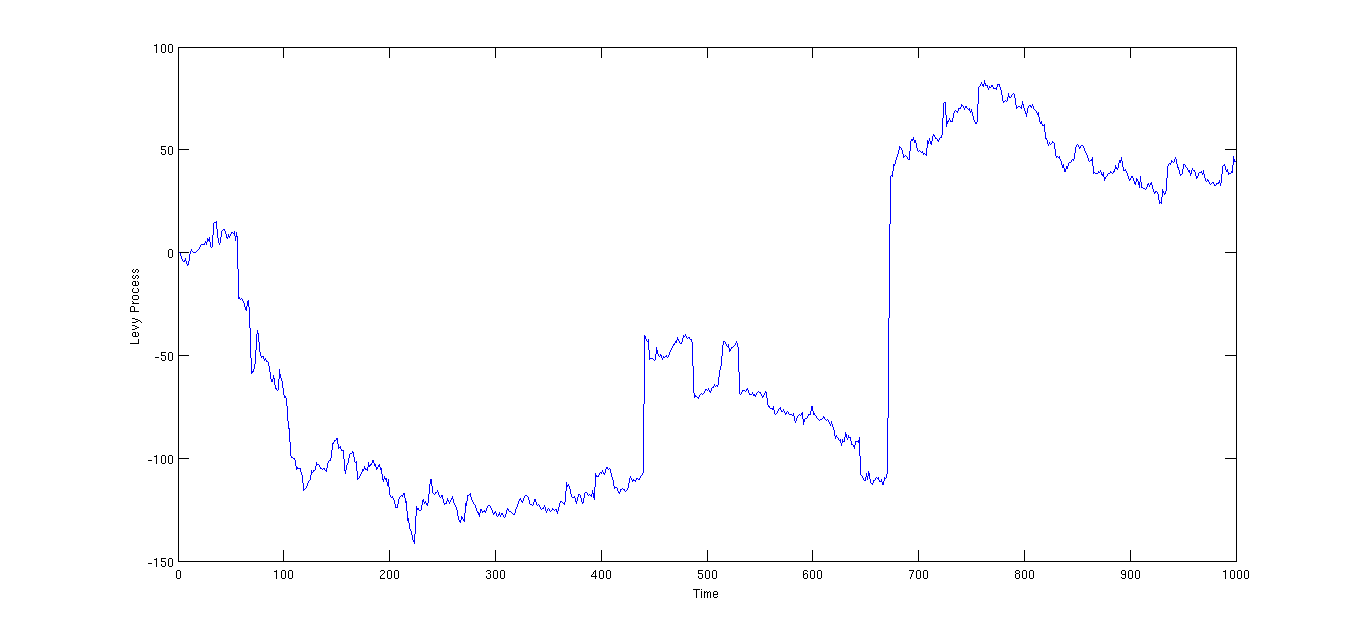
\includegraphics[width=1\linewidth]{levymotion_sample}}
		
		\caption{Path of the Levy motion for $\alpha = 1.5$}
	\end{figure}
\newpage
To observe and interesting fact of the Levy motion, let's denote $q_p(t)$ as a quantile of order \textit{p}. Then ($X(t)$ is Levy motion):
\begin{align*} 
P(X(t) < q_p(t)) = p  \\ 
P(X(1) < t^{\frac{-1}{\alpha}}q_p(t)) = p
\end{align*}
We can see that:
\begin{equation*}
q_p(1) = t^{\frac{-1}{\alpha}}q_p(t)
\end{equation*}
Figure 12 presents empirical and theoretical quantile lines for Levy process as well as sample path.

	\begin{figure}[h]
		\xput[0.5]{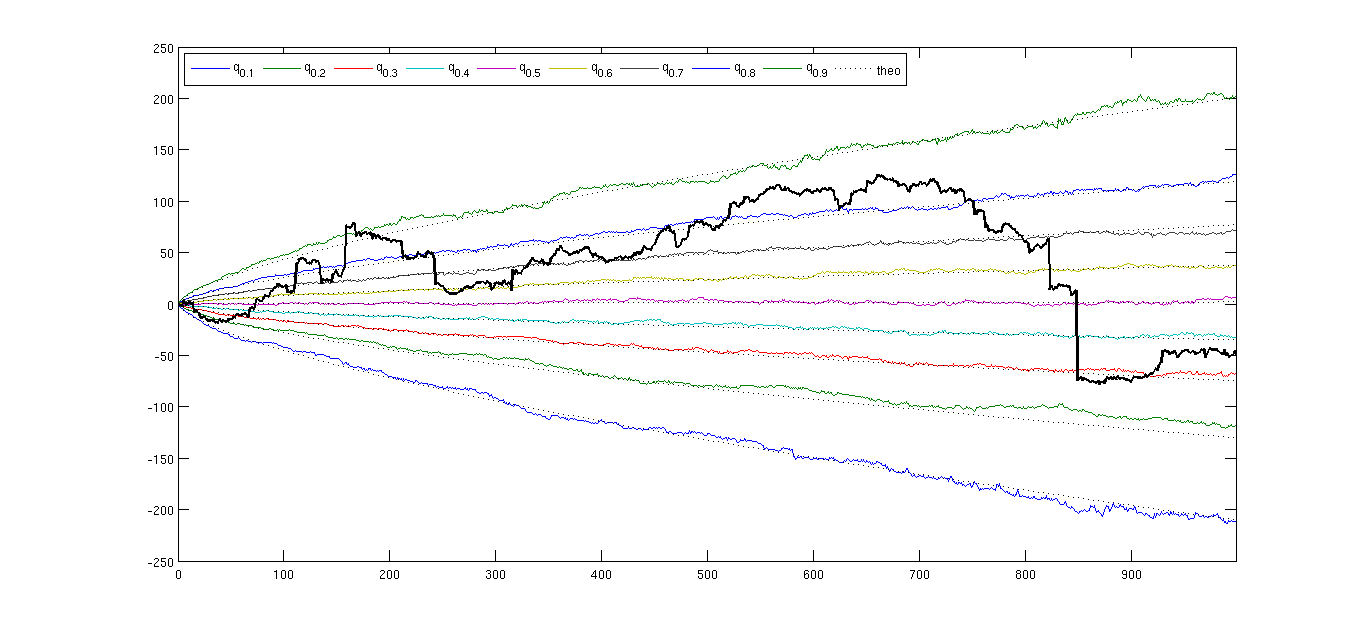
\includegraphics[width=1.5\linewidth]{levymotion_quantiles}}
		
		\caption{Quantile lines for Levy motion. Black line - sample path}
	\end{figure}

\subsection{Lamperti transformation}
We would like to work on self-similar processes, as they are invariant under suitable translations of time and scale. To obtain such process, we use Lamperti transformation, that changes stationary process to the corresponding self-similar one in the following way\footnote{[4]}:
\subparagraph{Lamperti transformaton}
\textit{If $Y = Y(t)$ is a stationary process and if for some $H > 0$:}
\begin{equation*}
X(t) = t^H Y(log(t)), \qquad for \qquad t > 0, \qquad X(0) = 0
\end{equation*}
\textit{Then $X = X(t)$ is H-ss} \\
Figure 13 presents quantile lines of Lamperti transformation of $\alpha$-stable process; it is clear, that they are parallel - they do not change in time, as well as distribution.\\

	\begin{figure}[h]
		\xput[0.5]{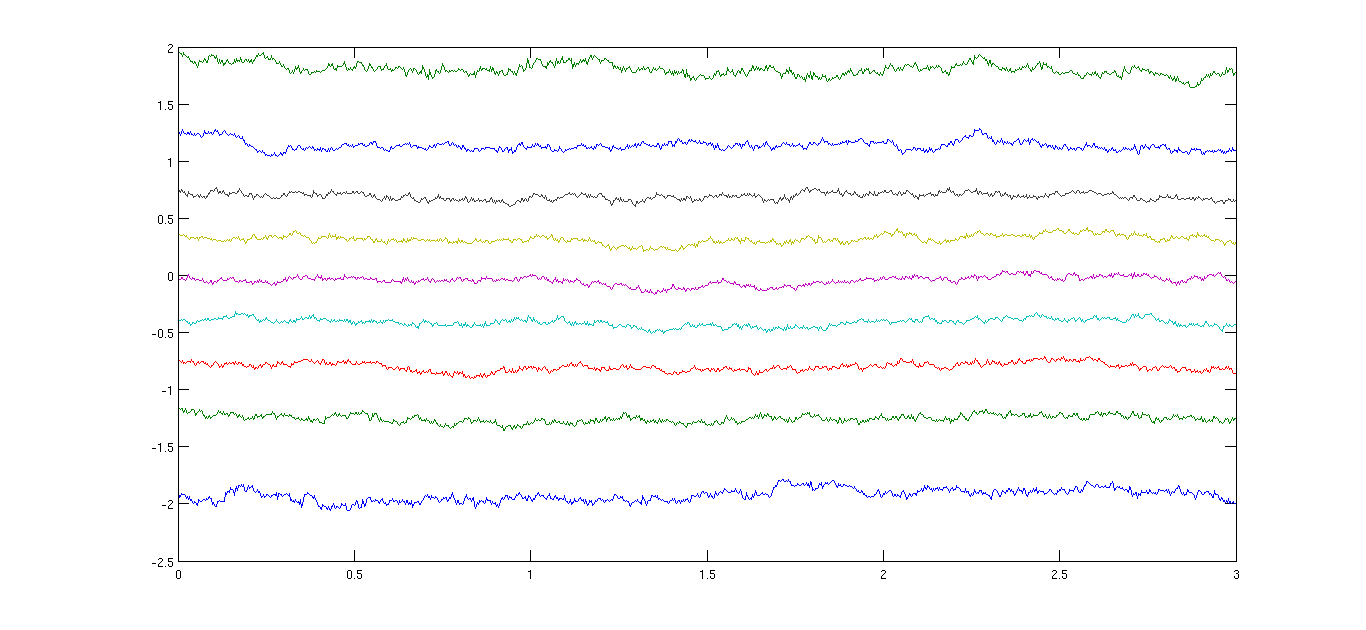
\includegraphics[width=1.5\linewidth]{qlines_stable}}
		
		\caption{Quantile lines for Lamperti transformation}
	\end{figure}
Next picture presents quantile lines for Orstein-Uhlenbeck process - we see that this process is asymptotically stationary.

	\begin{figure}[h]
		\xput[0.5]{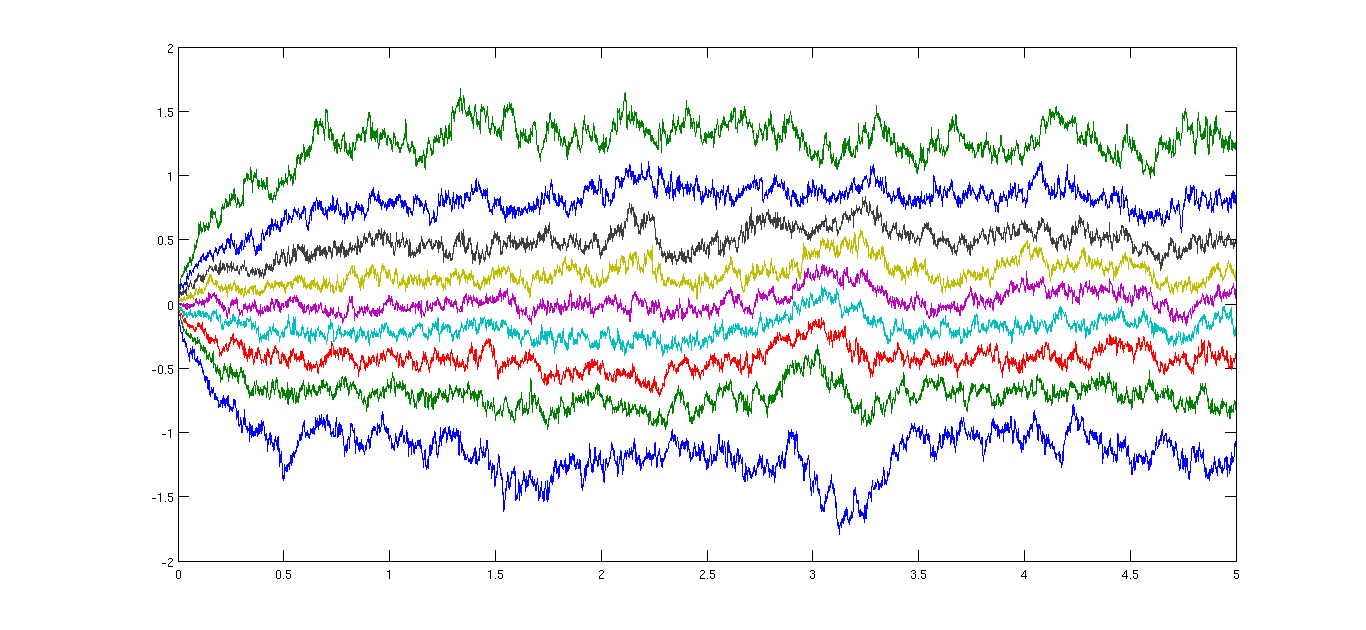
\includegraphics[width=1.5\linewidth]{qlines_OU}}
		
		\caption{Quantile lines for Orstein-Uhlenbeck process}
	\end{figure}
\newpage
\subsection{Fractional Brownian Motion}
One of the most interesting self-similar processes is fractional Brownian motion (fBm). The most characteristic for it it it's covariance function:
\begin{equation*}
E[B_H(t)B_H(s)] = \frac{1}{2}(|t|^{2H} + |s|^{2H} - |t-s|^{2H})
\end{equation*}
For $H = \frac{1}{2}$, it is a Brownian motion. Increments of the process are positively correlated for $H > \frac{1}{2}$ and negative correlated for $H < \frac{1}{2}$.\\
Increments of fBm, called Gaussian noise can have long range dependence (for $H > \frac{1}{2}$).\\
Figure 15 shows sample paths of fBm for different H; figure 16 shows corresponding autocorrelation functions.\\
As we can see from Figure 15, the lower value of H-index the more process is oscillating around mean.
	\begin{figure}[h]
		\xput[0.5]{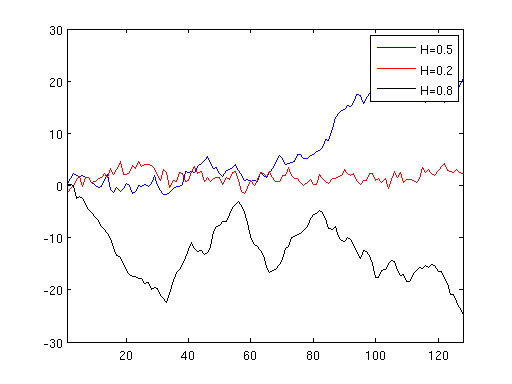
\includegraphics[width=0.9\linewidth]{fbm2}}
		
		\caption{Sample paths of fBm}
	\end{figure}
	
\begin{figure}[h]
		\xput[0.5]{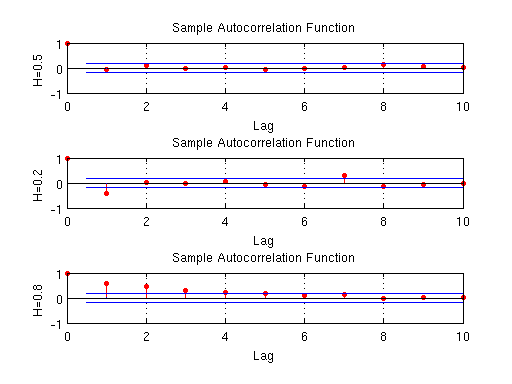
\includegraphics[width=0.9\linewidth]{autocorr}}
		
		\caption{Autocorrelation functions}
\end{figure}
\clearpage

\section{Estimation of parameters}
In this section we will estimate sample parameters and compare to theoretical ones.
\subsection{$\alpha$ parameters}
There are many method to estimate $\alpha$ parameter. Here we will use FLOM\footnote{[5]}, as it is simple and easy to understand.\\
Whole derivation of formulas can be found in proper document. Here we are interested with following ones:
\begin{align*}
L_2 &= \mathbf{E} [(log|X| - \mathbf{E}[log|X|)^2] ] \\
\psi_1 &= \frac{\pi^2}{6} \\
\alpha = ( (\frac{L_2}{\psi_1} - \frac{1}{2}) - \psi_1)^{\frac{1}{2}}
\end{align*}
Using this, we can check how this method estimate $\alpha$ from our sample. For each value of alpha, 100 vectors of stable random variables of length 1000 has generated. With formulas above, 100 estimators for each value of $\alpha$ has been obtained. Below we can see boxplots of that, as well as Mean Squared Error (MSE). We can see, that for large value (greater than 1.5) of $\alpha$, error becomes very significant - variance becomes very large.

\begin{figure}[h]
		\xput[0.5]{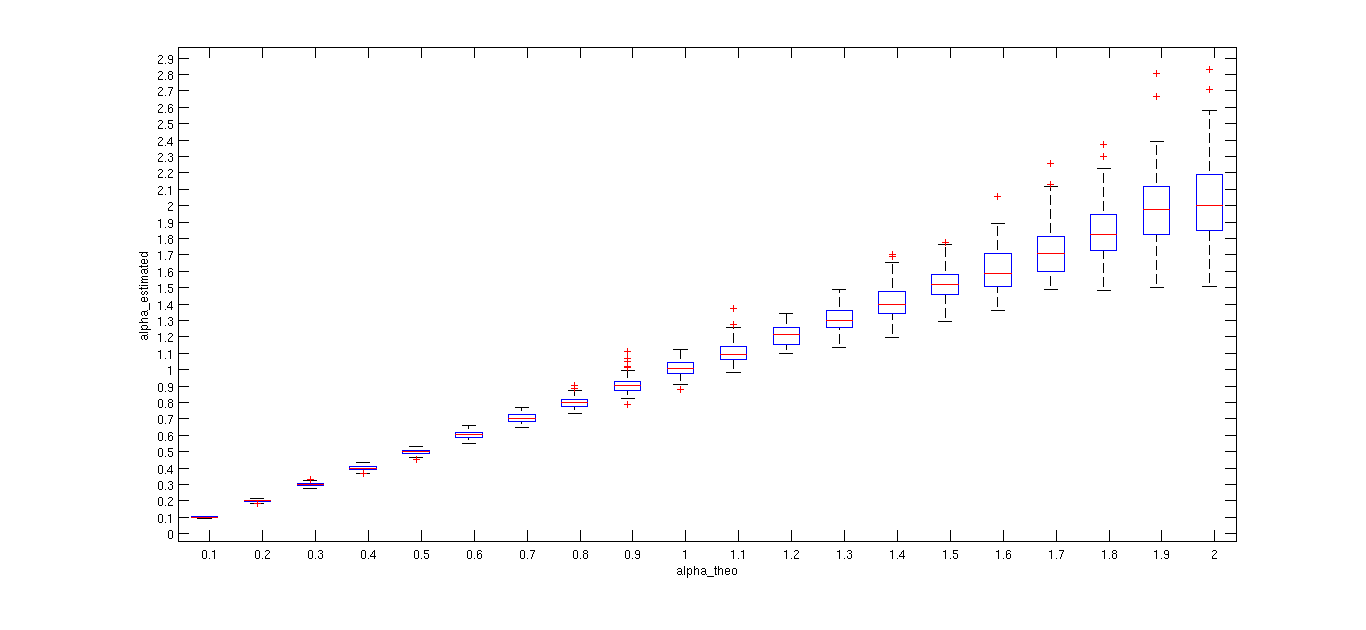
\includegraphics[width=1.3\linewidth]{alpha_est_boxplot}}
		
		\caption{Boxplots of $\alpha$}
\end{figure}

\begin{figure}[h]
		\xput[0.5]{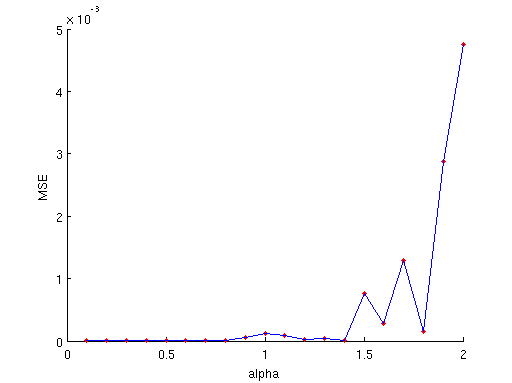
\includegraphics[width=1.1\linewidth]{alpha_est_MSE}}
		
		\caption{MSE of our parameter}
\end{figure}
\clearpage
\section{Bibliography}
[1] Stable Distributions, Models for Heavy Tailed Data; John P. Nolan; 2014 

[2] Stable Non-Gaussian Random Processes; G. Samorodnitsky, M.S. Taqqu; 1994 

[3] An overview of multivariate stable distributions; John P. Nolan; 2008 

[4] The Lamperti Transformation for Self-Similar Processes; K. Burnecki, M. Maejima, A. Weron; 1997

[5] Estimation of the Parameters of Skewed $alpha$-Stable Distributions; Ch. R. Dance; 1999
\end{document}
	